\documentclass[twoside]{book}

% Packages required by doxygen
\usepackage{fixltx2e}
\usepackage{calc}
\usepackage{doxygen}
\usepackage[export]{adjustbox} % also loads graphicx
\usepackage{graphicx}
\usepackage[utf8]{inputenc}
\usepackage{makeidx}
\usepackage{multicol}
\usepackage{multirow}
\PassOptionsToPackage{warn}{textcomp}
\usepackage{textcomp}
\usepackage[nointegrals]{wasysym}
\usepackage[table]{xcolor}

% Font selection
\usepackage[T1]{fontenc}
\usepackage[scaled=.90]{helvet}
\usepackage{courier}
\usepackage{amssymb}
\usepackage{sectsty}
\renewcommand{\familydefault}{\sfdefault}
\allsectionsfont{%
  \fontseries{bc}\selectfont%
  \color{darkgray}%
}
\renewcommand{\DoxyLabelFont}{%
  \fontseries{bc}\selectfont%
  \color{darkgray}%
}
\newcommand{\+}{\discretionary{\mbox{\scriptsize$\hookleftarrow$}}{}{}}

% Page & text layout
\usepackage{geometry}
\geometry{%
  a4paper,%
  top=2.5cm,%
  bottom=2.5cm,%
  left=2.5cm,%
  right=2.5cm%
}
\tolerance=750
\hfuzz=15pt
\hbadness=750
\setlength{\emergencystretch}{15pt}
\setlength{\parindent}{0cm}
\setlength{\parskip}{3ex plus 2ex minus 2ex}
\makeatletter
\renewcommand{\paragraph}{%
  \@startsection{paragraph}{4}{0ex}{-1.0ex}{1.0ex}{%
    \normalfont\normalsize\bfseries\SS@parafont%
  }%
}
\renewcommand{\subparagraph}{%
  \@startsection{subparagraph}{5}{0ex}{-1.0ex}{1.0ex}{%
    \normalfont\normalsize\bfseries\SS@subparafont%
  }%
}
\makeatother

% Headers & footers
\usepackage{fancyhdr}
\pagestyle{fancyplain}
\fancyhead[LE]{\fancyplain{}{\bfseries\thepage}}
\fancyhead[CE]{\fancyplain{}{}}
\fancyhead[RE]{\fancyplain{}{\bfseries\leftmark}}
\fancyhead[LO]{\fancyplain{}{\bfseries\rightmark}}
\fancyhead[CO]{\fancyplain{}{}}
\fancyhead[RO]{\fancyplain{}{\bfseries\thepage}}
\fancyfoot[LE]{\fancyplain{}{}}
\fancyfoot[CE]{\fancyplain{}{}}
\fancyfoot[RE]{\fancyplain{}{\bfseries\scriptsize 制作者 Doxygen }}
\fancyfoot[LO]{\fancyplain{}{\bfseries\scriptsize 制作者 Doxygen }}
\fancyfoot[CO]{\fancyplain{}{}}
\fancyfoot[RO]{\fancyplain{}{}}
\renewcommand{\footrulewidth}{0.4pt}
\renewcommand{\chaptermark}[1]{%
  \markboth{#1}{}%
}
\renewcommand{\sectionmark}[1]{%
  \markright{\thesection\ #1}%
}

% Indices & bibliography
\usepackage{natbib}
\usepackage[titles]{tocloft}
\setcounter{tocdepth}{3}
\setcounter{secnumdepth}{5}
\makeindex

% Hyperlinks (required, but should be loaded last)
\usepackage{ifpdf}
\ifpdf
  \usepackage[pdftex,pagebackref=true]{hyperref}
\else
  \usepackage[ps2pdf,pagebackref=true]{hyperref}
\fi
\hypersetup{%
  colorlinks=true,%
  linkcolor=blue,%
  citecolor=blue,%
  unicode%
}

% Custom commands
\newcommand{\clearemptydoublepage}{%
  \newpage{\pagestyle{empty}\cleardoublepage}%
}

\usepackage{caption}
\captionsetup{labelsep=space,justification=centering,font={bf},singlelinecheck=off,skip=4pt,position=top}

%===== C O N T E N T S =====

\begin{document}

% Titlepage & ToC
\hypersetup{pageanchor=false,
             bookmarksnumbered=true,
             pdfencoding=unicode
            }
\pagenumbering{alph}
\begin{titlepage}
\vspace*{7cm}
\begin{center}%
{\Large Doxy }\\
\vspace*{1cm}
{\large 制作者 Doxygen 1.8.13}\\
\end{center}
\end{titlepage}
\clearemptydoublepage
\pagenumbering{roman}
\tableofcontents
\clearemptydoublepage
\pagenumbering{arabic}
\hypersetup{pageanchor=true}

%--- Begin generated contents ---
\chapter{工程概览}
\label{index}\hypertarget{index}{}\begin{DoxyAuthor}{作者}
phae 
\end{DoxyAuthor}


邮箱 

\href{mailto:phae@lhlover.com}{\tt phae@lhlover.\+com} \begin{DoxyVersion}{版本}
1.\+0.\+0 
\end{DoxyVersion}
\begin{DoxyDate}{日期}
2022-\/06-\/20 
\end{DoxyDate}

\chapter{第一步,生成默认文档}
\label{md_doxygen}
\Hypertarget{md_doxygen}

\begin{DoxyCode}
doxygen -g
#或者不带注释的默认文档
doxygen -s -g
\end{DoxyCode}


\subsubsection*{第二步,修改配置文档}

\subsubsection*{第三步,填写注释}

\subsubsection*{第四步,程序文档生成}


\begin{DoxyCode}
#如果修改了Doxyfile名字,则在生成的Doxyfile所在的路径, 输入
doxygen your-cfg-filename

#如果没有修改名字的话,就是
doxygen Doxyfile
\end{DoxyCode}
 
\chapter{目录结构}
\label{md_README}
\Hypertarget{md_README}

\begin{DoxyCode}
Cmake+Doxygen
├── bin
│   └── main
├── build
├── build.sh
├── CMakeLists.txt
├── cmake
│   └── build\_doxygen.cmake
├── docs
│   ├── install.sh
│   ├── Doxygen.in
│   └── doxygen
│   │   ├── html
│   │   └── latex
├── Doxyfile
├── doxygen.md
├── src
│   ├── main.cpp
│   ├── Message.cpp
│   └── Message.hpp
├── thirdparty
│   └── dbg
│   │   └── dbg.hpp
└── README.md
\end{DoxyCode}



\begin{DoxyItemize}
\item {\bfseries bin\+:} 用于存放生成的可执行文件
\item {\bfseries bin/main\+:} 生成的可执行文件
\item {\bfseries build \+:} 用于存放build时cmake产生的中间文件
\item {\bfseries build.\+sh \+:} build脚本文件。
\item {\bfseries C\+Make\+Lists.\+txt \+:} cmake文件。
\item {\bfseries cmake \+:} 用于存放其他的cmake文件。
\item {\bfseries cmake/build\+\_\+doxygen.\+cmake \+:} 生成doxygen的cmake文件。
\item {\bfseries Doxyfile \+:} 由cmake构建生成的\+Doxygen文件
\item {\bfseries doxygen.\+md \+:} doxygen相关的说明文件。
\item {\bfseries docs \+:} 用于存放项目的相关文档。
\item {\bfseries docs/install.\+sh \+:} 安装doxygen的脚本文件。
\item {\bfseries docs/\+Doxygen.\+in \+:} build\+\_\+doxygen.\+cmake中引用的\+Doxygen.\+in,供cmake生成\+Doxygen文件。
\item {\bfseries src\+:} 用于存放源文件。
\item {\bfseries thirdparty \+:} 用于存放第三方库,每个第三库以单独目录的形式组织在thirdparty 目录下。
\item {\bfseries R\+E\+A\+D\+M\+E.\+md \+:} 工程说明文件。 
\end{DoxyItemize}
\chapter{Bug 列表}
\label{bug}
\Hypertarget{bug}

\begin{DoxyRefList}
\item[\label{bug__bug000001}%
\Hypertarget{bug__bug000001}%
类 \hyperlink{classMessage}{Message} ]Not all memory is freed when deleting an object of this class. 
\end{DoxyRefList}
\chapter{继承关系索引}
\section{类继承关系}
此继承关系列表按字典顺序粗略的排序\+: \begin{DoxyCompactList}
\item \contentsline{section}{dbg\+:\+:Debug\+Output}{\pageref{classdbg_1_1DebugOutput}}{}
\item \contentsline{section}{dbg\+:\+:detail\+\_\+detector\+:\+:detector$<$ Default, Always\+Void, Op, Args $>$}{\pageref{structdbg_1_1detail__detector_1_1detector}}{}
\item \contentsline{section}{dbg\+:\+:detail\+\_\+detector\+:\+:detector$<$ Default, void\+\_\+t$<$ Op$<$ Args... $>$ $>$, Op, Args... $>$}{\pageref{structdbg_1_1detail__detector_1_1detector_3_01Default_00_01void__t_3_01Op_3_01Args_8_8_8_01_4_01_4_00_01Op_00_01Args_8_8_8_01_4}}{}
\item \contentsline{section}{dbg\+:\+:detail\+:\+:is\+\_\+container$<$ T $>$}{\pageref{structdbg_1_1detail_1_1is__container}}{}
\item is\+\_\+detected\begin{DoxyCompactList}
\item \contentsline{section}{dbg\+:\+:detail\+:\+:has\+\_\+ostream\+\_\+operator$<$ T $>$}{\pageref{structdbg_1_1detail_1_1has__ostream__operator}}{}
\end{DoxyCompactList}
\item \contentsline{section}{dbg\+:\+:last$<$ T, U $>$}{\pageref{structdbg_1_1last}}{}
\item \contentsline{section}{dbg\+:\+:last$<$ T $>$}{\pageref{structdbg_1_1last_3_01T_01_4}}{}
\item \contentsline{section}{Message}{\pageref{classMessage}}{}
\item \contentsline{section}{dbg\+:\+:detail\+\_\+detector\+:\+:nonesuch}{\pageref{structdbg_1_1detail__detector_1_1nonesuch}}{}
\item \contentsline{section}{dbg\+:\+:pretty\+\_\+print\+\_\+tuple$<$ Idx $>$}{\pageref{structdbg_1_1pretty__print__tuple}}{}
\item \contentsline{section}{dbg\+:\+:pretty\+\_\+print\+\_\+tuple$<$ 0 $>$}{\pageref{structdbg_1_1pretty__print__tuple_3_010_01_4}}{}
\item \contentsline{section}{dbg\+:\+:print\+\_\+formatted$<$ T $>$}{\pageref{structdbg_1_1print__formatted}}{}
\item \contentsline{section}{dbg\+:\+:print\+\_\+type$<$ T $>$}{\pageref{structdbg_1_1print__type}}{}
\item \contentsline{section}{dbg\+:\+:time}{\pageref{structdbg_1_1time}}{}
\item \contentsline{section}{dbg\+:\+:type\+\_\+tag$<$ T $>$}{\pageref{structdbg_1_1type__tag}}{}
\end{DoxyCompactList}

\chapter{类索引}
\section{类列表}
这里列出了所有类、结构、联合以及接口定义等,并附带简要说明\+:\begin{DoxyCompactList}
\item\contentsline{section}{\hyperlink{classdbg_1_1DebugOutput}{dbg\+::\+Debug\+Output} }{\pageref{classdbg_1_1DebugOutput}}{}
\item\contentsline{section}{\hyperlink{structdbg_1_1detail__detector_1_1detector}{dbg\+::detail\+\_\+detector\+::detector$<$ Default, Always\+Void, Op, Args $>$} }{\pageref{structdbg_1_1detail__detector_1_1detector}}{}
\item\contentsline{section}{\hyperlink{structdbg_1_1detail__detector_1_1detector_3_01Default_00_01void__t_3_01Op_3_01Args_8_8_8_01_4_01_4_00_01Op_00_01Args_8_8_8_01_4}{dbg\+::detail\+\_\+detector\+::detector$<$ Default, void\+\_\+t$<$ Op$<$ Args... $>$ $>$, Op, Args... $>$} }{\pageref{structdbg_1_1detail__detector_1_1detector_3_01Default_00_01void__t_3_01Op_3_01Args_8_8_8_01_4_01_4_00_01Op_00_01Args_8_8_8_01_4}}{}
\item\contentsline{section}{\hyperlink{structdbg_1_1detail_1_1has__ostream__operator}{dbg\+::detail\+::has\+\_\+ostream\+\_\+operator$<$ T $>$} }{\pageref{structdbg_1_1detail_1_1has__ostream__operator}}{}
\item\contentsline{section}{\hyperlink{structdbg_1_1detail_1_1is__container}{dbg\+::detail\+::is\+\_\+container$<$ T $>$} }{\pageref{structdbg_1_1detail_1_1is__container}}{}
\item\contentsline{section}{\hyperlink{structdbg_1_1last}{dbg\+::last$<$ T, U $>$} }{\pageref{structdbg_1_1last}}{}
\item\contentsline{section}{\hyperlink{structdbg_1_1last_3_01T_01_4}{dbg\+::last$<$ T $>$} }{\pageref{structdbg_1_1last_3_01T_01_4}}{}
\item\contentsline{section}{\hyperlink{classMessage}{Message} \\*Pretty nice class }{\pageref{classMessage}}{}
\item\contentsline{section}{\hyperlink{structdbg_1_1detail__detector_1_1nonesuch}{dbg\+::detail\+\_\+detector\+::nonesuch} }{\pageref{structdbg_1_1detail__detector_1_1nonesuch}}{}
\item\contentsline{section}{\hyperlink{structdbg_1_1pretty__print__tuple}{dbg\+::pretty\+\_\+print\+\_\+tuple$<$ Idx $>$} }{\pageref{structdbg_1_1pretty__print__tuple}}{}
\item\contentsline{section}{\hyperlink{structdbg_1_1pretty__print__tuple_3_010_01_4}{dbg\+::pretty\+\_\+print\+\_\+tuple$<$ 0 $>$} }{\pageref{structdbg_1_1pretty__print__tuple_3_010_01_4}}{}
\item\contentsline{section}{\hyperlink{structdbg_1_1print__formatted}{dbg\+::print\+\_\+formatted$<$ T $>$} }{\pageref{structdbg_1_1print__formatted}}{}
\item\contentsline{section}{\hyperlink{structdbg_1_1print__type}{dbg\+::print\+\_\+type$<$ T $>$} }{\pageref{structdbg_1_1print__type}}{}
\item\contentsline{section}{\hyperlink{structdbg_1_1time}{dbg\+::time} }{\pageref{structdbg_1_1time}}{}
\item\contentsline{section}{\hyperlink{structdbg_1_1type__tag}{dbg\+::type\+\_\+tag$<$ T $>$} }{\pageref{structdbg_1_1type__tag}}{}
\end{DoxyCompactList}

\chapter{文件索引}
\section{文件列表}
这里列出了所有文档化的文件,并附带简要说明\+:\begin{DoxyCompactList}
\item\contentsline{section}{src/\hyperlink{main_8cpp}{main.\+cpp} \\*测试头文件 }{\pageref{main_8cpp}}{}
\item\contentsline{section}{src/{\bfseries Message.\+hpp} }{\pageref{Message_8hpp}}{}
\item\contentsline{section}{thirdparty/dbg/{\bfseries dbg.\+hpp} }{\pageref{dbg_8hpp}}{}
\end{DoxyCompactList}

\chapter{类说明}
\hypertarget{classdbg_1_1DebugOutput}{}\section{dbg\+:\+:Debug\+Output类 参考}
\label{classdbg_1_1DebugOutput}\index{dbg\+::\+Debug\+Output@{dbg\+::\+Debug\+Output}}
\subsection*{Public 类型}
\begin{DoxyCompactItemize}
\item 
\mbox{\Hypertarget{classdbg_1_1DebugOutput_a5d9b38d5b9276cb584c0e20e9b1a2045}\label{classdbg_1_1DebugOutput_a5d9b38d5b9276cb584c0e20e9b1a2045}} 
using {\bfseries expr\+\_\+t} = const char $\ast$
\end{DoxyCompactItemize}
\subsection*{Public 成员函数}
\begin{DoxyCompactItemize}
\item 
\mbox{\Hypertarget{classdbg_1_1DebugOutput_a7bb0378758aa1006e2423eff57ee36a2}\label{classdbg_1_1DebugOutput_a7bb0378758aa1006e2423eff57ee36a2}} 
{\bfseries Debug\+Output} (const char $\ast$filepath, int line, const char $\ast$function\+\_\+name)
\item 
\mbox{\Hypertarget{classdbg_1_1DebugOutput_aa135787802db4a6b0b4eb185185e13ca}\label{classdbg_1_1DebugOutput_aa135787802db4a6b0b4eb185185e13ca}} 
{\footnotesize template$<$typename... T$>$ }\\auto {\bfseries print} (std\+::initializer\+\_\+list$<$ expr\+\_\+t $>$ exprs, std\+::initializer\+\_\+list$<$ std\+::string $>$ types, T \&\&... values) -\/$>$ last\+\_\+t$<$ T... $>$
\end{DoxyCompactItemize}


该类的文档由以下文件生成\+:\begin{DoxyCompactItemize}
\item 
thirdparty/dbg/dbg.\+hpp\end{DoxyCompactItemize}

\hypertarget{structdbg_1_1detail__detector_1_1detector}{}\section{dbg\+:\+:detail\+\_\+detector\+:\+:detector$<$ Default, Always\+Void, Op, Args $>$ 模板结构体 参考}
\label{structdbg_1_1detail__detector_1_1detector}\index{dbg\+::detail\+\_\+detector\+::detector$<$ Default, Always\+Void, Op, Args $>$@{dbg\+::detail\+\_\+detector\+::detector$<$ Default, Always\+Void, Op, Args $>$}}
\subsection*{Public 类型}
\begin{DoxyCompactItemize}
\item 
\mbox{\Hypertarget{structdbg_1_1detail__detector_1_1detector_af1b6da4282d723669e926c52f446a989}\label{structdbg_1_1detail__detector_1_1detector_af1b6da4282d723669e926c52f446a989}} 
using {\bfseries value\+\_\+t} = std\+::false\+\_\+type
\item 
\mbox{\Hypertarget{structdbg_1_1detail__detector_1_1detector_aab6b446944545683b9533ea8fc623480}\label{structdbg_1_1detail__detector_1_1detector_aab6b446944545683b9533ea8fc623480}} 
using {\bfseries type} = Default
\end{DoxyCompactItemize}


该结构体的文档由以下文件生成\+:\begin{DoxyCompactItemize}
\item 
thirdparty/dbg/dbg.\+hpp\end{DoxyCompactItemize}

\hypertarget{structdbg_1_1detail__detector_1_1detector_3_01Default_00_01void__t_3_01Op_3_01Args_8_8_8_01_4_01_4_00_01Op_00_01Args_8_8_8_01_4}{}\section{dbg\+:\+:detail\+\_\+detector\+:\+:detector$<$ Default, void\+\_\+t$<$ Op$<$ Args... $>$ $>$, Op, Args... $>$ 模板结构体 参考}
\label{structdbg_1_1detail__detector_1_1detector_3_01Default_00_01void__t_3_01Op_3_01Args_8_8_8_01_4_01_4_00_01Op_00_01Args_8_8_8_01_4}\index{dbg\+::detail\+\_\+detector\+::detector$<$ Default, void\+\_\+t$<$ Op$<$ Args... $>$ $>$, Op, Args... $>$@{dbg\+::detail\+\_\+detector\+::detector$<$ Default, void\+\_\+t$<$ Op$<$ Args... $>$ $>$, Op, Args... $>$}}
\subsection*{Public 类型}
\begin{DoxyCompactItemize}
\item 
\mbox{\Hypertarget{structdbg_1_1detail__detector_1_1detector_3_01Default_00_01void__t_3_01Op_3_01Args_8_8_8_01_4_01_4_00_01Op_00_01Args_8_8_8_01_4_ab9dc20c0565be267d2d98b0e0f4a565b}\label{structdbg_1_1detail__detector_1_1detector_3_01Default_00_01void__t_3_01Op_3_01Args_8_8_8_01_4_01_4_00_01Op_00_01Args_8_8_8_01_4_ab9dc20c0565be267d2d98b0e0f4a565b}} 
using {\bfseries value\+\_\+t} = std\+::true\+\_\+type
\item 
\mbox{\Hypertarget{structdbg_1_1detail__detector_1_1detector_3_01Default_00_01void__t_3_01Op_3_01Args_8_8_8_01_4_01_4_00_01Op_00_01Args_8_8_8_01_4_a2119ba35e684b8292286546a1cea10d1}\label{structdbg_1_1detail__detector_1_1detector_3_01Default_00_01void__t_3_01Op_3_01Args_8_8_8_01_4_01_4_00_01Op_00_01Args_8_8_8_01_4_a2119ba35e684b8292286546a1cea10d1}} 
using {\bfseries type} = Op$<$ Args... $>$
\end{DoxyCompactItemize}


该结构体的文档由以下文件生成\+:\begin{DoxyCompactItemize}
\item 
thirdparty/dbg/dbg.\+hpp\end{DoxyCompactItemize}

\hypertarget{structdbg_1_1detail_1_1has__ostream__operator}{}\section{dbg\+:\+:detail\+:\+:has\+\_\+ostream\+\_\+operator$<$ T $>$ 模板结构体 参考}
\label{structdbg_1_1detail_1_1has__ostream__operator}\index{dbg\+::detail\+::has\+\_\+ostream\+\_\+operator$<$ T $>$@{dbg\+::detail\+::has\+\_\+ostream\+\_\+operator$<$ T $>$}}


类 dbg\+:\+:detail\+:\+:has\+\_\+ostream\+\_\+operator$<$ T $>$ 继承关系图\+:
\nopagebreak
\begin{figure}[H]
\begin{center}
\leavevmode
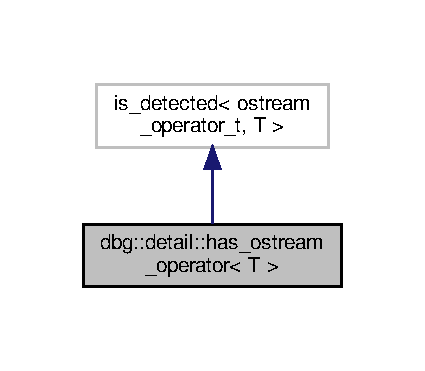
\includegraphics[width=204pt]{structdbg_1_1detail_1_1has__ostream__operator__inherit__graph}
\end{center}
\end{figure}


dbg\+:\+:detail\+:\+:has\+\_\+ostream\+\_\+operator$<$ T $>$ 的协作图\+:
\nopagebreak
\begin{figure}[H]
\begin{center}
\leavevmode
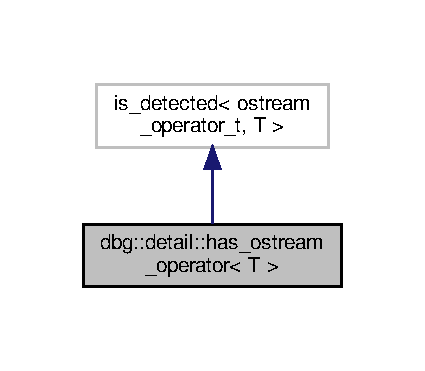
\includegraphics[width=204pt]{structdbg_1_1detail_1_1has__ostream__operator__coll__graph}
\end{center}
\end{figure}


该结构体的文档由以下文件生成\+:\begin{DoxyCompactItemize}
\item 
thirdparty/dbg/dbg.\+hpp\end{DoxyCompactItemize}

\hypertarget{structdbg_1_1detail_1_1is__container}{}\section{dbg\+:\+:detail\+:\+:is\+\_\+container$<$ T $>$ 模板结构体 参考}
\label{structdbg_1_1detail_1_1is__container}\index{dbg\+::detail\+::is\+\_\+container$<$ T $>$@{dbg\+::detail\+::is\+\_\+container$<$ T $>$}}
\subsection*{静态 Public 属性}
\begin{DoxyCompactItemize}
\item 
static constexpr bool {\bfseries value}
\end{DoxyCompactItemize}


\subsection{类成员变量说明}
\mbox{\Hypertarget{structdbg_1_1detail_1_1is__container_aa9a4594488352384b65b36198ac414f8}\label{structdbg_1_1detail_1_1is__container_aa9a4594488352384b65b36198ac414f8}} 
\index{dbg\+::detail\+::is\+\_\+container@{dbg\+::detail\+::is\+\_\+container}!value@{value}}
\index{value@{value}!dbg\+::detail\+::is\+\_\+container@{dbg\+::detail\+::is\+\_\+container}}
\subsubsection{\texorpdfstring{value}{value}}
{\footnotesize\ttfamily template$<$typename T $>$ \\
constexpr bool \hyperlink{structdbg_1_1detail_1_1is__container}{dbg\+::detail\+::is\+\_\+container}$<$ T $>$\+::value\hspace{0.3cm}{\ttfamily [static]}}

{\bfseries 初始值\+:}
\begin{DoxyCode}
=
      is\_detected<detect\_begin\_t, T>::value &&
      is\_detected<detect\_end\_t, T>::value &&
      is\_detected<detect\_size\_t, T>::value &&
      !std::is\_same<std::string,
                    \textcolor{keyword}{typename} std::remove\_cv<
                        \textcolor{keyword}{typename} std::remove\_reference<T>::type>::type>::value
\end{DoxyCode}


该结构体的文档由以下文件生成\+:\begin{DoxyCompactItemize}
\item 
thirdparty/dbg/dbg.\+hpp\end{DoxyCompactItemize}

\hypertarget{structdbg_1_1last}{}\section{dbg\+:\+:last$<$ T, U $>$ 模板结构体 参考}
\label{structdbg_1_1last}\index{dbg\+::last$<$ T, U $>$@{dbg\+::last$<$ T, U $>$}}
\subsection*{Public 类型}
\begin{DoxyCompactItemize}
\item 
\mbox{\Hypertarget{structdbg_1_1last_aac2d6dd66fecfc0f3f37ecb4a02b0779}\label{structdbg_1_1last_aac2d6dd66fecfc0f3f37ecb4a02b0779}} 
using {\bfseries type} = typename \hyperlink{structdbg_1_1last}{last}$<$ U... $>$\+::type
\end{DoxyCompactItemize}


该结构体的文档由以下文件生成\+:\begin{DoxyCompactItemize}
\item 
thirdparty/dbg/dbg.\+hpp\end{DoxyCompactItemize}

\hypertarget{structdbg_1_1last_3_01T_01_4}{}\section{dbg\+:\+:last$<$ T $>$ 模板结构体 参考}
\label{structdbg_1_1last_3_01T_01_4}\index{dbg\+::last$<$ T $>$@{dbg\+::last$<$ T $>$}}
\subsection*{Public 类型}
\begin{DoxyCompactItemize}
\item 
\mbox{\Hypertarget{structdbg_1_1last_3_01T_01_4_a6715c2f60dfaa8a096517ce45ff43999}\label{structdbg_1_1last_3_01T_01_4_a6715c2f60dfaa8a096517ce45ff43999}} 
using {\bfseries type} = T
\end{DoxyCompactItemize}


该结构体的文档由以下文件生成\+:\begin{DoxyCompactItemize}
\item 
thirdparty/dbg/dbg.\+hpp\end{DoxyCompactItemize}

\hypertarget{classMessage}{}\section{Message类 参考}
\label{classMessage}\index{Message@{Message}}


Pretty nice class.  




{\ttfamily \#include $<$Message.\+hpp$>$}

\subsection*{Public 成员函数}
\begin{DoxyCompactItemize}
\item 
\hyperlink{classMessage_a2246f9e3015883a76b7a0249c80604ec}{Message} (const std\+::string \&m)
\begin{DoxyCompactList}\small\item\em Constructor from a string \end{DoxyCompactList}\item 
\hyperlink{classMessage_ab165b08f675163c9fde8ed2da0c18d3a}{Message} (const char $\ast$m)
\begin{DoxyCompactList}\small\item\em Constructor from a character array \end{DoxyCompactList}\end{DoxyCompactItemize}
\subsection*{友元}
\begin{DoxyCompactItemize}
\item 
\mbox{\Hypertarget{classMessage_a6cac7113816180f023230f8dfd14633a}\label{classMessage_a6cac7113816180f023230f8dfd14633a}} 
std\+::ostream \& {\bfseries operator$<$$<$} (std\+::ostream \&os, \hyperlink{classMessage}{Message} \&obj)
\end{DoxyCompactItemize}


\subsection{详细描述}
Pretty nice class. 

This class is used to demonstrate a number of section commands. \begin{DoxyAuthor}{作者}
John Doe 

Jan Doe 
\end{DoxyAuthor}
\begin{DoxyVersion}{版本}
4.\+1a 
\end{DoxyVersion}
\begin{DoxyDate}{日期}
1990-\/2011 
\end{DoxyDate}
\begin{DoxyPrecond}{前置条件}
First initialize the system. 
\end{DoxyPrecond}
\begin{DoxyRefDesc}{Bug}
\item[\hyperlink{bug__bug000001}{Bug}]Not all memory is freed when deleting an object of this class. \end{DoxyRefDesc}
\begin{DoxyWarning}{警告}
Improper use can crash your application 
\end{DoxyWarning}
\begin{DoxyCopyright}{版权所有}
G\+NU Public License. 
\end{DoxyCopyright}


\subsection{构造及析构函数说明}
\mbox{\Hypertarget{classMessage_a2246f9e3015883a76b7a0249c80604ec}\label{classMessage_a2246f9e3015883a76b7a0249c80604ec}} 
\index{Message@{Message}!Message@{Message}}
\index{Message@{Message}!Message@{Message}}
\subsubsection{\texorpdfstring{Message()}{Message()}\hspace{0.1cm}{\footnotesize\ttfamily [1/2]}}
{\footnotesize\ttfamily Message\+::\+Message (\begin{DoxyParamCaption}\item[{const std\+::string \&}]{m }\end{DoxyParamCaption})\hspace{0.3cm}{\ttfamily [inline]}}



Constructor from a string 


\begin{DoxyParams}[1]{参数}
\mbox{\tt in}  & {\em m} & a message \\
\hline
\end{DoxyParams}
\mbox{\Hypertarget{classMessage_ab165b08f675163c9fde8ed2da0c18d3a}\label{classMessage_ab165b08f675163c9fde8ed2da0c18d3a}} 
\index{Message@{Message}!Message@{Message}}
\index{Message@{Message}!Message@{Message}}
\subsubsection{\texorpdfstring{Message()}{Message()}\hspace{0.1cm}{\footnotesize\ttfamily [2/2]}}
{\footnotesize\ttfamily Message\+::\+Message (\begin{DoxyParamCaption}\item[{const char $\ast$}]{m }\end{DoxyParamCaption})\hspace{0.3cm}{\ttfamily [inline]}}



Constructor from a character array 


\begin{DoxyParams}[1]{参数}
\mbox{\tt in}  & {\em m} & a message \\
\hline
\end{DoxyParams}


该类的文档由以下文件生成\+:\begin{DoxyCompactItemize}
\item 
src/Message.\+hpp\item 
src/Message.\+cpp\end{DoxyCompactItemize}

\hypertarget{structdbg_1_1detail__detector_1_1nonesuch}{}\section{dbg\+:\+:detail\+\_\+detector\+:\+:nonesuch结构体 参考}
\label{structdbg_1_1detail__detector_1_1nonesuch}\index{dbg\+::detail\+\_\+detector\+::nonesuch@{dbg\+::detail\+\_\+detector\+::nonesuch}}
\subsection*{Public 成员函数}
\begin{DoxyCompactItemize}
\item 
\mbox{\Hypertarget{structdbg_1_1detail__detector_1_1nonesuch_a82c9bfc90b56b542819d8df5af7cebe6}\label{structdbg_1_1detail__detector_1_1nonesuch_a82c9bfc90b56b542819d8df5af7cebe6}} 
{\bfseries nonesuch} (\hyperlink{structdbg_1_1detail__detector_1_1nonesuch}{nonesuch} const \&)=delete
\item 
\mbox{\Hypertarget{structdbg_1_1detail__detector_1_1nonesuch_af0d1b2ab32ace678e2c9d95684d1917b}\label{structdbg_1_1detail__detector_1_1nonesuch_af0d1b2ab32ace678e2c9d95684d1917b}} 
void {\bfseries operator=} (\hyperlink{structdbg_1_1detail__detector_1_1nonesuch}{nonesuch} const \&)=delete
\end{DoxyCompactItemize}


该结构体的文档由以下文件生成\+:\begin{DoxyCompactItemize}
\item 
thirdparty/dbg/dbg.\+hpp\end{DoxyCompactItemize}

\hypertarget{structdbg_1_1pretty__print__tuple}{}\section{dbg\+:\+:pretty\+\_\+print\+\_\+tuple$<$ Idx $>$ 模板结构体 参考}
\label{structdbg_1_1pretty__print__tuple}\index{dbg\+::pretty\+\_\+print\+\_\+tuple$<$ Idx $>$@{dbg\+::pretty\+\_\+print\+\_\+tuple$<$ Idx $>$}}
\subsection*{静态 Public 成员函数}
\begin{DoxyCompactItemize}
\item 
\mbox{\Hypertarget{structdbg_1_1pretty__print__tuple_a17c2bca6c330e88da2082efa4c3a9be5}\label{structdbg_1_1pretty__print__tuple_a17c2bca6c330e88da2082efa4c3a9be5}} 
{\footnotesize template$<$typename... Ts$>$ }\\static void {\bfseries print} (std\+::ostream \&stream, const std\+::tuple$<$ Ts... $>$ \&tuple)
\end{DoxyCompactItemize}


该结构体的文档由以下文件生成\+:\begin{DoxyCompactItemize}
\item 
thirdparty/dbg/dbg.\+hpp\end{DoxyCompactItemize}

\hypertarget{structdbg_1_1pretty__print__tuple_3_010_01_4}{}\section{dbg\+:\+:pretty\+\_\+print\+\_\+tuple$<$ 0 $>$ 模板结构体 参考}
\label{structdbg_1_1pretty__print__tuple_3_010_01_4}\index{dbg\+::pretty\+\_\+print\+\_\+tuple$<$ 0 $>$@{dbg\+::pretty\+\_\+print\+\_\+tuple$<$ 0 $>$}}
\subsection*{静态 Public 成员函数}
\begin{DoxyCompactItemize}
\item 
\mbox{\Hypertarget{structdbg_1_1pretty__print__tuple_3_010_01_4_a9961147d35a3bcc6b89af9610c68ad39}\label{structdbg_1_1pretty__print__tuple_3_010_01_4_a9961147d35a3bcc6b89af9610c68ad39}} 
{\footnotesize template$<$typename... Ts$>$ }\\static void {\bfseries print} (std\+::ostream \&stream, const std\+::tuple$<$ Ts... $>$ \&tuple)
\end{DoxyCompactItemize}


该结构体的文档由以下文件生成\+:\begin{DoxyCompactItemize}
\item 
thirdparty/dbg/dbg.\+hpp\end{DoxyCompactItemize}

\hypertarget{structdbg_1_1print__formatted}{}\section{dbg\+:\+:print\+\_\+formatted$<$ T $>$ 模板结构体 参考}
\label{structdbg_1_1print__formatted}\index{dbg\+::print\+\_\+formatted$<$ T $>$@{dbg\+::print\+\_\+formatted$<$ T $>$}}
\subsection*{Public 成员函数}
\begin{DoxyCompactItemize}
\item 
\mbox{\Hypertarget{structdbg_1_1print__formatted_a77fef2b6aa871171bfefe58bab8a03fe}\label{structdbg_1_1print__formatted_a77fef2b6aa871171bfefe58bab8a03fe}} 
{\bfseries print\+\_\+formatted} (T value, int numeric\+\_\+base)
\item 
\mbox{\Hypertarget{structdbg_1_1print__formatted_ab6a7c4280acb807f5c5ab812f80a8aca}\label{structdbg_1_1print__formatted_ab6a7c4280acb807f5c5ab812f80a8aca}} 
{\bfseries operator T} () const
\item 
\mbox{\Hypertarget{structdbg_1_1print__formatted_ab490d37d984d053177b6af3f94d0136e}\label{structdbg_1_1print__formatted_ab490d37d984d053177b6af3f94d0136e}} 
const char $\ast$ {\bfseries prefix} () const
\end{DoxyCompactItemize}
\subsection*{Public 属性}
\begin{DoxyCompactItemize}
\item 
\mbox{\Hypertarget{structdbg_1_1print__formatted_a080056e4f7af0c86ed46bc2ecb9c6f1e}\label{structdbg_1_1print__formatted_a080056e4f7af0c86ed46bc2ecb9c6f1e}} 
T {\bfseries inner}
\item 
\mbox{\Hypertarget{structdbg_1_1print__formatted_af57ecb89743fca9b4cb1d0afd3c9d9f4}\label{structdbg_1_1print__formatted_af57ecb89743fca9b4cb1d0afd3c9d9f4}} 
int {\bfseries base}
\end{DoxyCompactItemize}


该结构体的文档由以下文件生成\+:\begin{DoxyCompactItemize}
\item 
thirdparty/dbg/dbg.\+hpp\end{DoxyCompactItemize}

\hypertarget{structdbg_1_1print__type}{}\section{dbg\+:\+:print\+\_\+type$<$ T $>$ 模板结构体 参考}
\label{structdbg_1_1print__type}\index{dbg\+::print\+\_\+type$<$ T $>$@{dbg\+::print\+\_\+type$<$ T $>$}}


该结构体的文档由以下文件生成\+:\begin{DoxyCompactItemize}
\item 
thirdparty/dbg/dbg.\+hpp\end{DoxyCompactItemize}

\hypertarget{structdbg_1_1time}{}\section{dbg\+:\+:time结构体 参考}
\label{structdbg_1_1time}\index{dbg\+::time@{dbg\+::time}}


该结构体的文档由以下文件生成\+:\begin{DoxyCompactItemize}
\item 
thirdparty/dbg/dbg.\+hpp\end{DoxyCompactItemize}

\hypertarget{structdbg_1_1type__tag}{}\section{dbg\+:\+:type\+\_\+tag$<$ T $>$ 模板结构体 参考}
\label{structdbg_1_1type__tag}\index{dbg\+::type\+\_\+tag$<$ T $>$@{dbg\+::type\+\_\+tag$<$ T $>$}}


该结构体的文档由以下文件生成\+:\begin{DoxyCompactItemize}
\item 
thirdparty/dbg/dbg.\+hpp\end{DoxyCompactItemize}

\chapter{文件说明}
\hypertarget{main_8cpp}{}\section{src/main.cpp 文件参考}
\label{main_8cpp}\index{src/main.\+cpp@{src/main.\+cpp}}


测试头文件  


{\ttfamily \#include \char`\"{}Message.\+hpp\char`\"{}}\newline
{\ttfamily \#include \char`\"{}version.\+h\char`\"{}}\newline
{\ttfamily \#include $<$iostream$>$}\newline
main.\+cpp 的引用(Include)关系图\+:
\nopagebreak
\begin{figure}[H]
\begin{center}
\leavevmode
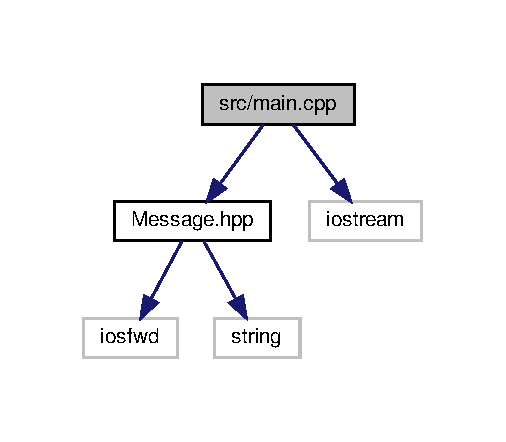
\includegraphics[width=316pt]{main_8cpp__incl}
\end{center}
\end{figure}
\subsection*{宏定义}
\begin{DoxyCompactItemize}
\item 
\mbox{\Hypertarget{main_8cpp_a8ffa8049026210b78ffb88ca997322a3}\label{main_8cpp_a8ffa8049026210b78ffb88ca997322a3}} 
\#define {\bfseries V\+E\+R\+S\+I\+O\+NS}~V\+E\+R\+S\+I\+O\+N\+\_\+\+M\+A\+J\+OR \char`\"{}.\char`\"{} V\+E\+R\+S\+I\+O\+N\+\_\+\+M\+I\+N\+OR \char`\"{}.\char`\"{} V\+E\+R\+S\+I\+O\+N\+\_\+\+P\+A\+T\+CH \char`\"{} \char`\"{} B\+U\+I\+L\+D\+\_\+\+T\+I\+M\+E\+S\+T\+A\+MP
\end{DoxyCompactItemize}
\subsection*{函数}
\begin{DoxyCompactItemize}
\item 
\mbox{\Hypertarget{main_8cpp_ae66f6b31b5ad750f1fe042a706a4e3d4}\label{main_8cpp_ae66f6b31b5ad750f1fe042a706a4e3d4}} 
int {\bfseries main} ()
\end{DoxyCompactItemize}


\subsection{详细描述}
测试头文件 

这个是测试\+Doxygen 
%--- End generated contents ---

% Index
\backmatter
\newpage
\phantomsection
\clearemptydoublepage
\addcontentsline{toc}{chapter}{索引}
\printindex

\end{document}
